%!TEX TS-program = xelatex
%!TEX encoding = UTF-8 Unicode
\documentclass[12pt, xcolor=dvipsnames]{beamer}
\definecolor{slight}{gray}{0.9}
\fboxsep=10pt
\usecolortheme[named=Royal Blue]{structure}
\useinnertheme{circles}
\usepackage[no-math]{fontspec}
\usepackage{xltxtra, xunicode}
\usepackage[utf8]{inputenc}
%\usepackage[sc, osf]{mathpazo}
\usepackage[minionint, lf, mathtabular]{MinionPro}
\setmainfont[Mapping=tex-text]{Minion Web Pro}
\setsansfont[Mapping=tex-text]{Myriad Web Pro}
\setmonofont[Scale=MatchLowercase]{Source Code Pro}
\usefonttheme{professionalfonts}
%% 中文字配置
\usepackage[
CJKmath=true, indentfirst=false, PunctStyle={quanjiao},
CheckSingle=true, SlantFont, BoldFont
]{xeCJK}
\setCJKmainfont[Scale=0.9, BoldFont=Hiragino Mincho ProN W6]{Hiragino Mincho ProN W3}
%\setCJKmainfont[Scale=0.9, BoldFont=Noto Sans CJK JP Bold]{Noto Sans CJK JP Medium}
\setCJKsansfont[Scale=0.9, BoldFont=Hiragino Sans W6]{Hiragino Sans W4}
%\setCJKsansfont[Scale=0.9, BoldFont=Hiragino Sans CNS W6]{Hiragino Sans CNS W3}
%\setCJKsansfont[Scale=0.9, BoldFont=Hiragino Sans W7]{Hiragino Sans W4}
%\setCJKsansfont[Scale=0.9, BoldFont=Source Han Sans UI TC Bold]{Source Han Sans UI TC Regular}
%\setCJKsansfont[Scale=0.9, BoldFont=PingFang TC Semibold]{PingFang TC Regular}
\setCJKmonofont[Scale=0.9, BoldFont=Yuanti TC Regular]{Hiragino Maru Gothic ProN W4}
\usepackage{fancyvrb, attachfile2, pstricks}
\usepackage{graphicx}
\setbeamerfont{page number in head/foot}{size=\tiny}
\setbeamertemplate{footline}[frame number]
\usepackage{xmpmulti, booktabs, multicol}
\setbeamertemplate{navigation symbols}{}
\let\WriteBookmarks\relax
\usepackage{dcolumn}
\newcolumntype{.}[1]{D{.}{.}{#1}}
\newcolumntype{,}[1]{D{,}{,}{#1}}

\linespread{1.25}

\setbeamersize{text margin left=.8em, text margin right=.6em}

\makeatletter
\defbeamertemplate{itemize item}{mycircle}{\LARGE\raise-1.6pt\hbox{\textbullet}}
\makeatother

\setbeamertemplate{itemize item}[mycircle]
\setbeamertemplate{itemize subitem}[triangle]
\setlength\leftmargini{1.3em}
\setlength\leftmarginii{1em}


%\CTXFR
\title{\bf{\Huge {}\\[-2mm] Principles of Economics \\[2mm] Review Session}}
\author{{\Large 張耕齊\\[2mm] Keng-Chi Chang}}
\institute{{}\\[-7mm]\footnotesize\tt{<r03323070@ntu.edu.tw>}\\[2mm]}
\date{\large 2016.11.23}
\begin{document}
\fontsize{12}{14pt}\selectfont

\begin{frame}
\titlepage
\end{frame}


\begin{frame}
\frametitle{\bf Circular-Flow Diagram}
\begin{center}
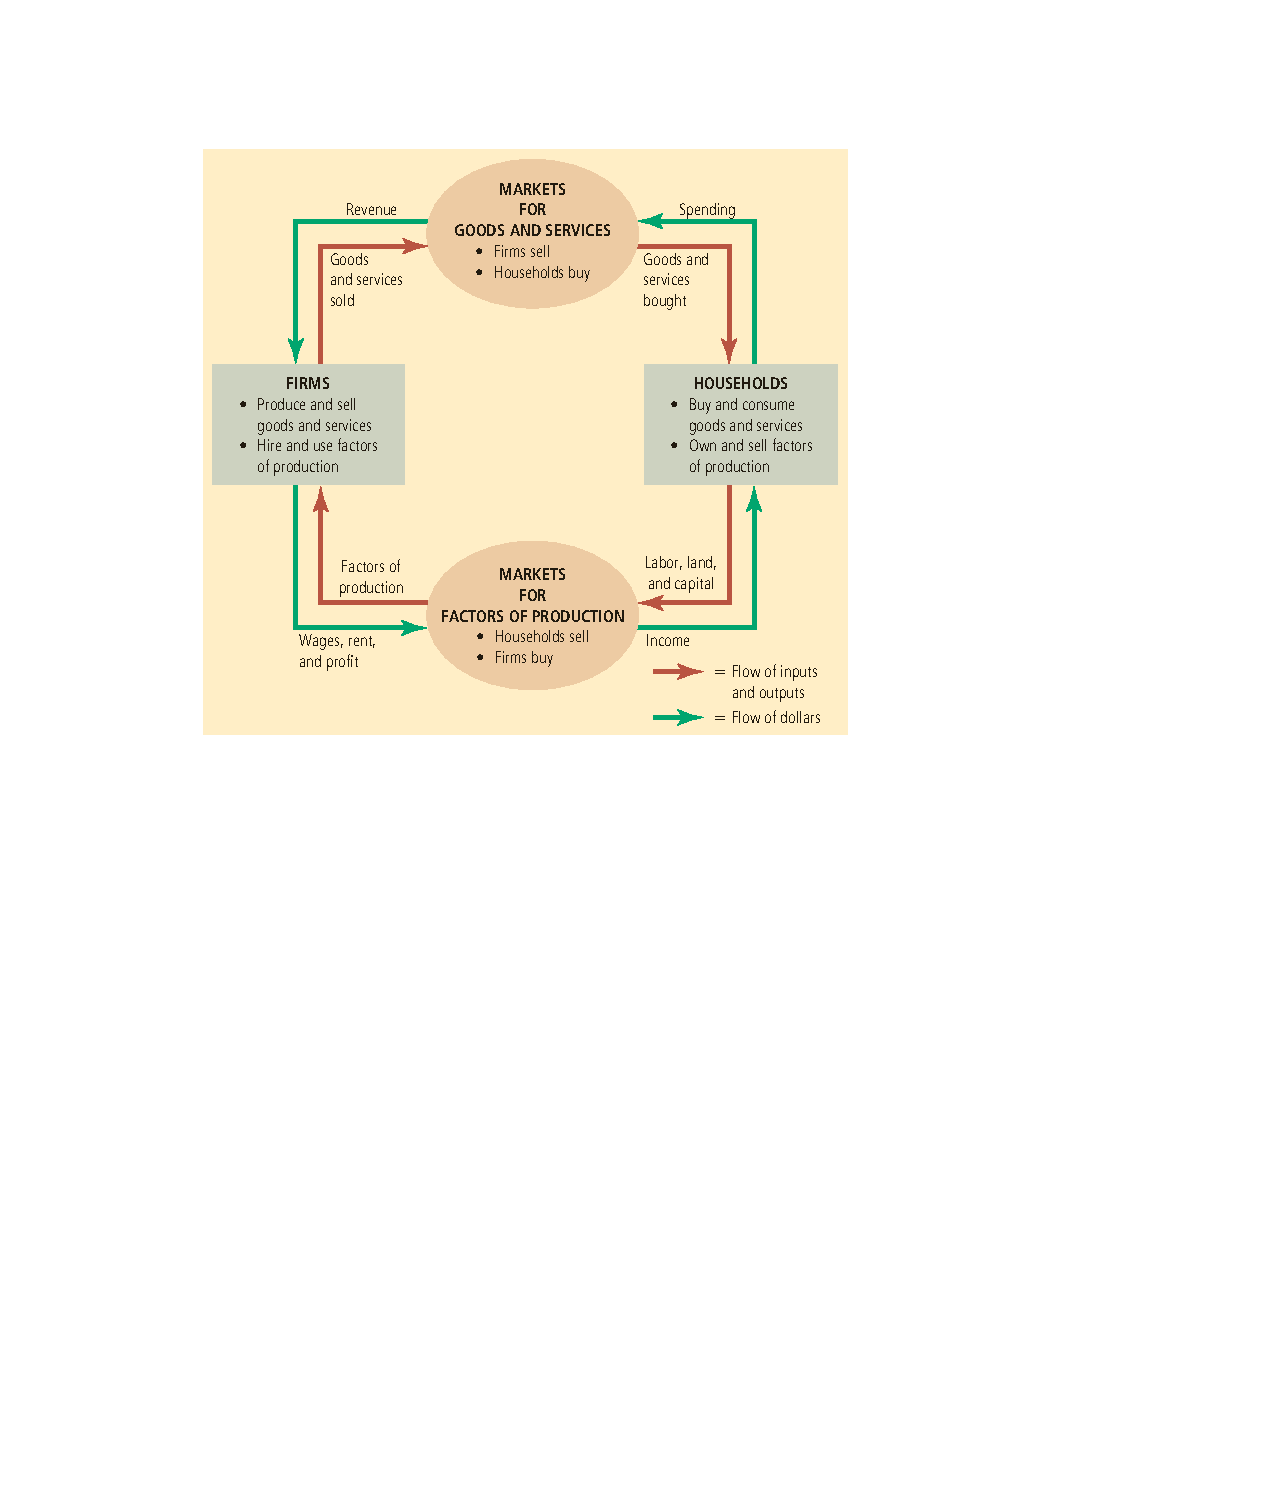
\includegraphics[height=.85\textheight]{figures/circular-flow.pdf}
\end{center}
\end{frame}



\begin{frame}
\frametitle{\bf §11.1 Demand for Factors of Production}
\begin{itemize}
\item Firms use labor and capital as inputs to produce goods as output
\item This is captured by the production function $Y=F(K,L)$
\item Firms can compute how an additional input will affect output, which is called the marginal product
\item If the firm wants to decide whether to hire an additional worker
\item MR of employing a worker is her value of marginal product
\item MC of employing a worker is the wage firm has to pay
\item In a competitive market, this is $P\times MPL=w$
\item Similarly, the demand for capital is determined by $P\times MPK=r$
\item Example: Cobb-Douglas production function $Y=K^\alpha L^{1-\alpha}$
\end{itemize}
\end{frame}


\begin{frame}
\frametitle{\bf Cobb-Douglas Production Function}
\begin{center}
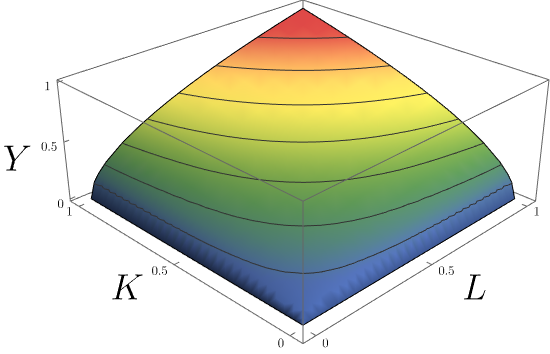
\includegraphics[width=\linewidth]{figures/Cobb_douglas.png}
\end{center}
\end{frame}


\begin{frame}
\frametitle{\bf Demand for Labor}
\textsf{\bfseries ALL 11-2.} 
For Acme Manufacturing, the marginal product of labor is \[MP = 160 - 3L.\] Acme is a perfect competitor and sells its output at a price of \$20 per unit. It also pays a wage of \$200 per worker. How many workers should Acme employ to maximize its profits?
\end{frame}


\begin{frame}
\frametitle{\bf §11.2 Supply of Labor}
\begin{itemize}
\item Suppose workers get utility from consumption and leisure
\item Workers face tradeoffs between going to work (so earning higher income and can consume more goods) and not going to work (so enjoys leisure time)
\item Workers maximize utility by choosing working hours such that wage equals the marginal benefit of leisure
\item By varying the wage rate, we can get the supply of labor
\end{itemize}
\end{frame}



\begin{frame}
\frametitle{\bf Supply of Labor}
\small \textsf{\bfseries ALL 11-6.} 
For a long time, your firm has been paying its workers a wage of \$20 per hour and your employees have been happy to work 40 hours per week at this wage. Business is suddenly booming and your firm would really like your workers to agree to a 50-hour work week in order to meet this new demand for your product. You are considering two strategies. Under the first, you would raise the wage for all hours worked from \$20 per hour to \$22 per hour; under the second, you would leave the wage for the first 40 hours per week at \$20 but offer \$30 per hour for hours worked above 40 hours (that is, you would offer time-and-a-half for overtime). Both strategies have the same cost of \$1,100 if a worker chooses to work 50 hours. Which strategy is more likely to lead your employees to agree to a 50-hour work week?
\end{frame}


\begin{frame}
\frametitle{\bf Labor Market}
\small \textsf{\bfseries Final 2009 Multiple Choice Q10.} 
Dan owns one of the many bakeries in New York City. Which of the following events will lead to an increase in Dan's demand for the services of bakers?
\begin{enumerate}\itemsep-0.5ex
\item[(i)] The price of muffins increases. (Muffins are Dan's specialty.)
\item[(ii)] Dan adds three new ovens to the kitchen area to help the bakers work faster.
\item[(iii)] Local bakers form a union to protect themselves from low wages.
\end{enumerate}
\end{frame}


\begin{frame}
\frametitle{\bf US Income Distribution}
\begin{center}
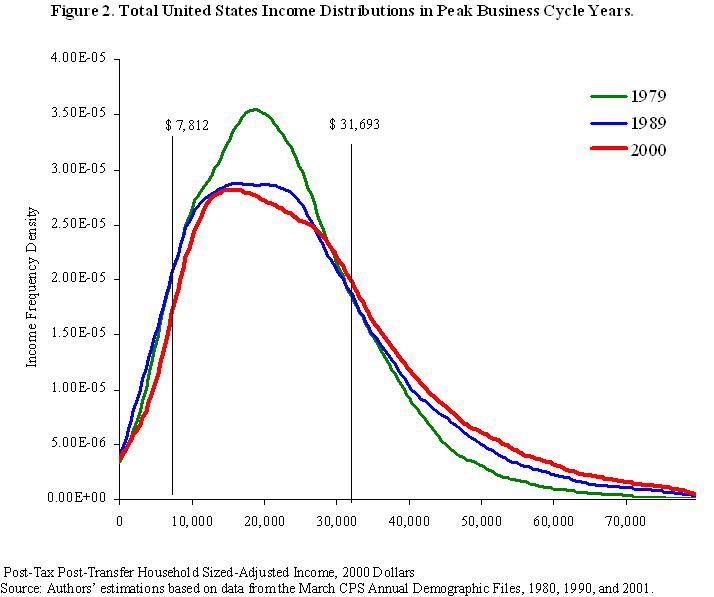
\includegraphics[height=.85\textheight]{figures/dist.jpg}
\end{center}
\end{frame}





\begin{frame}
\frametitle{\bf §11.3 Cross-Sectional Inequality}
\begin{itemize}
\item How to explain inequality for a certain time period?
\begin{itemize}
\item Human capital: Some people have more skill that is useful in the job market. Ex. college vs. high school graduates
\item Compensating wage differential: Some jobs are more risky and people want to avoid risk, so they get paid more Ex. Coal mining
\item Taste-based discrimination: Employers don't like certain people
\item Statistical discrimination: Employers form expectations for some types of people based on past experiences
\item Read \href{http://talkecon.com/discrimination/}{this article} if you are interested in discrimination
\item Superstar Phenomenon: Some industries have an extremely high demand for superstars. Ex. Sports, entertainments
\end{itemize}
\end{itemize}
\end{frame}



\begin{frame}
\frametitle{\bf US Wage Change Over Time}
\begin{center}
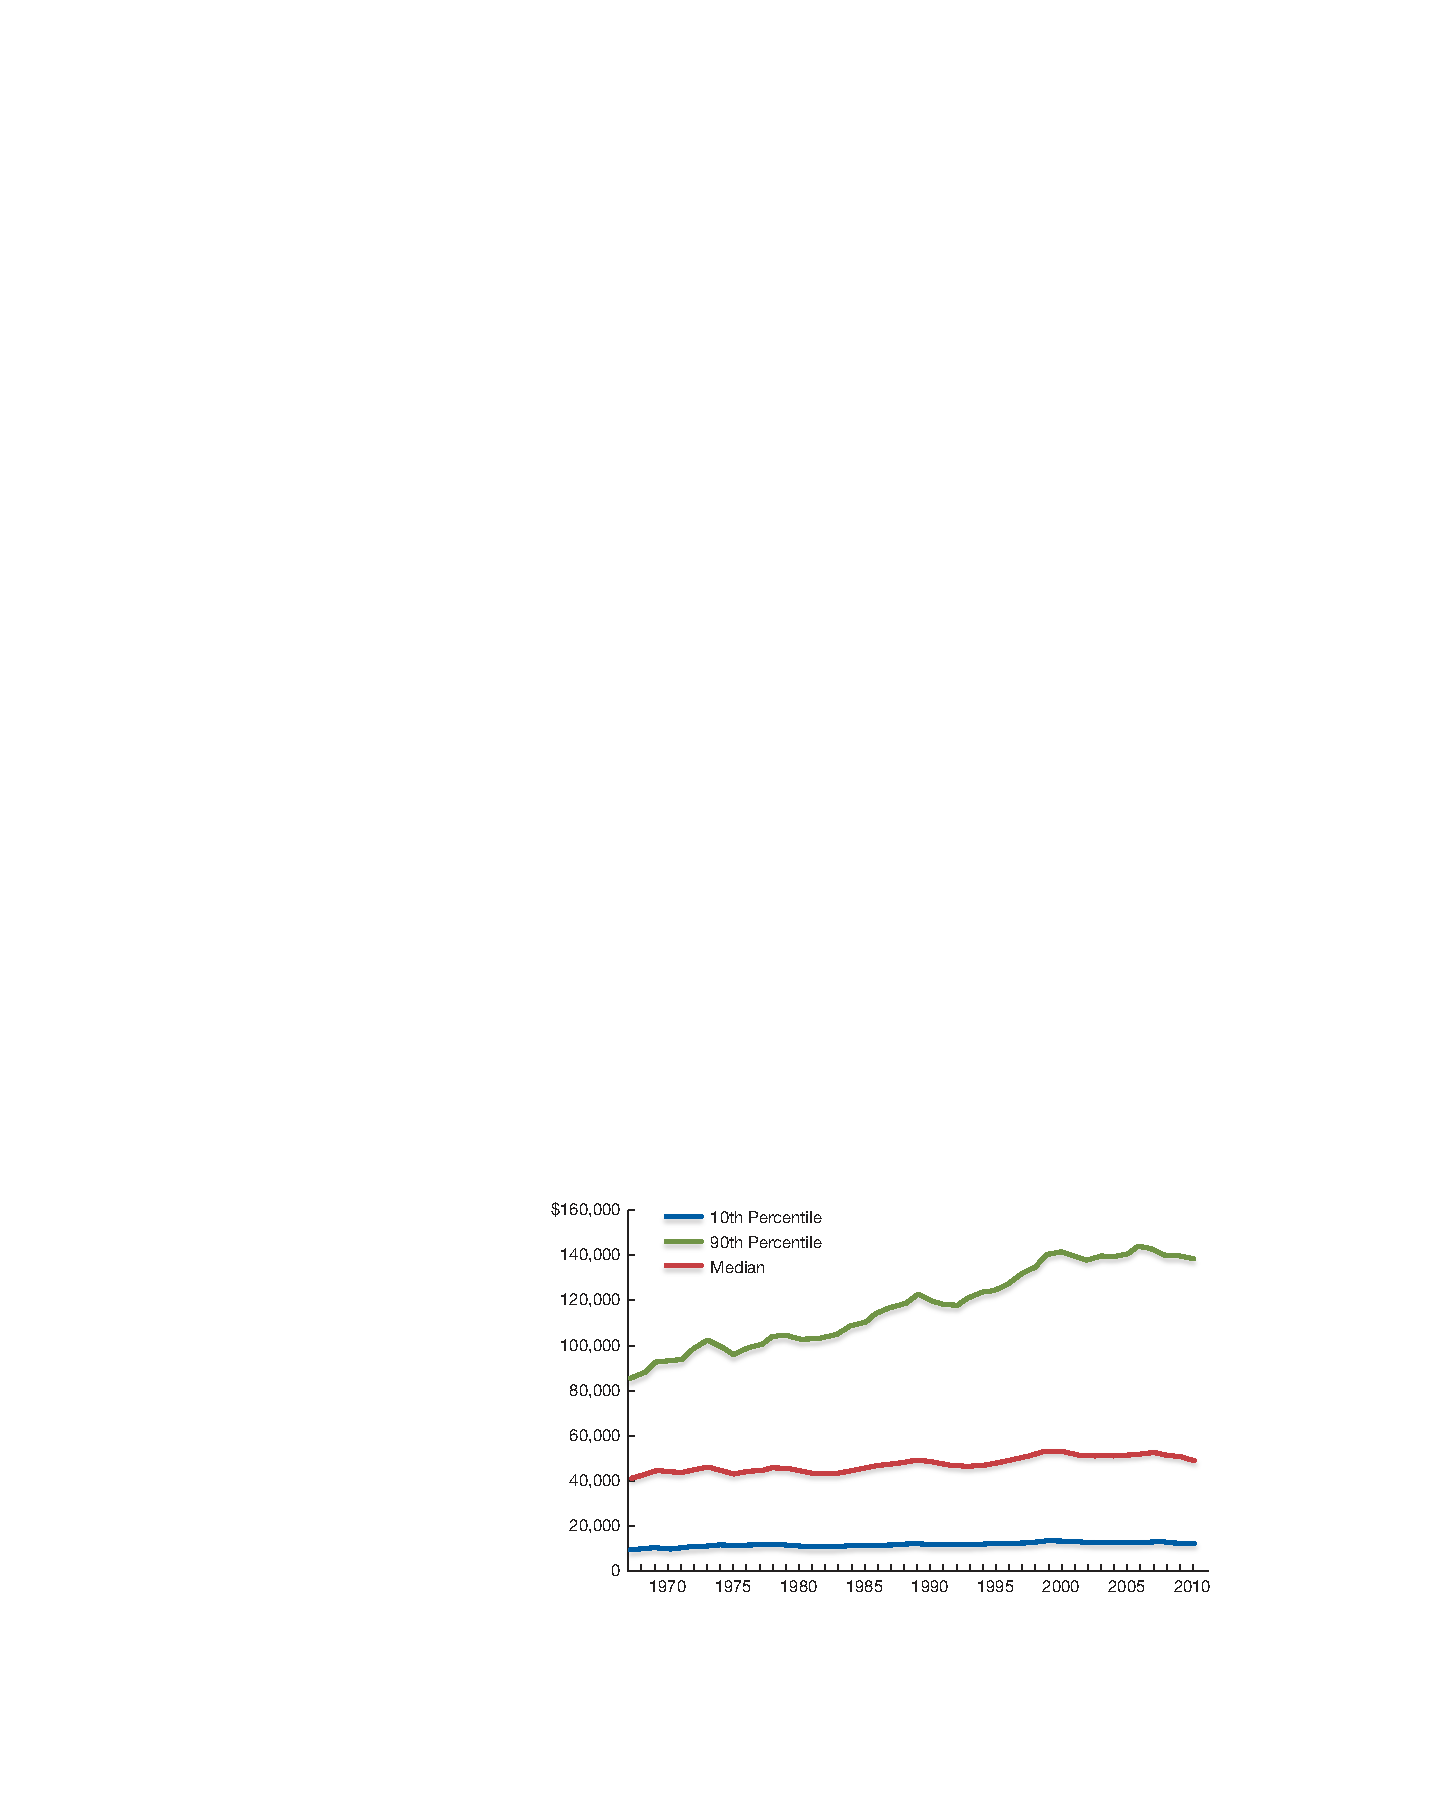
\includegraphics[width=\linewidth]{figures/1.pdf}
\end{center}
\end{frame}



\begin{frame}
\frametitle{\bf §11.3 Inequality Over Time}
\begin{itemize}
\item Why inequality seems to boost in the past few decades?
\begin{itemize}
\item Skill-biased technological change: Some technological change that is good for skilled labor but bad for unskilled labor so increases inequality. That is, it complements skilled labor but substitutes unskilled labor. So the relative demand for skilled worker vs. unskilled worker increases. Ex. Computer, Artificial Intelligence
\item Related concept: Labor-saving vs. labor-complementary technology
\item Skill-biased technological change is usually labor-saving for unskilled labor and labor-complementary for skilled labor
\item Globalization: Trade with China may hurt domestic working class and increases inequality, since workers in China substitutes domestic workers
\end{itemize}
\end{itemize}
\end{frame}



\begin{frame}
\begin{center}
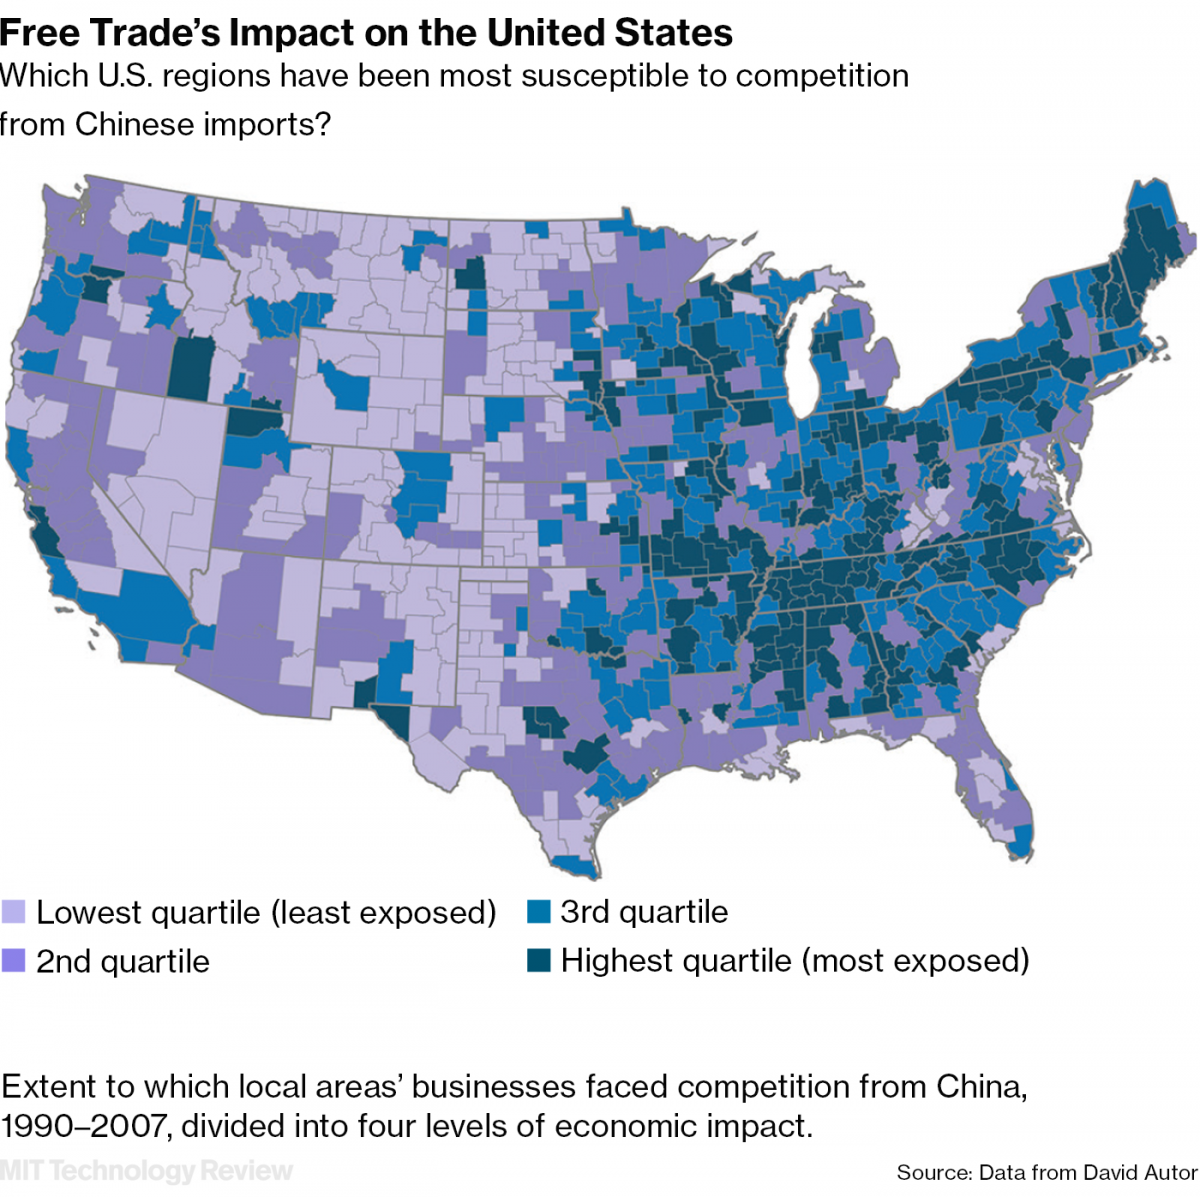
\includegraphics[height=\textheight]{figures/autor.png}
\end{center}
\end{frame}


\begin{frame}
\frametitle{\bf Inequality}
\small \textsf{\bfseries Final 2009 Multiple Choice Q11.} 
Which of the following is not an explanation for why better educated workers earn more, on
average, than less educated workers in the United States?
\begin{enumerate}\itemsep-0.5ex
\item[a.] Better educated workers have higher marginal productivities, on average.
\item[b.] Compensating differentials lower the wages of skilled workers relative to unskilled workers.
\item[c.] The United States tends to import goods produced with unskilled labor, which reduces the U.S. demand for unskilled labor.
\item[d.] The demand for skilled labor has risen over time relative to the demand for unskilled labor. 
\end{enumerate}
\end{frame}





\end{document}